\chapter{Lenguaje MC2}

MC2 es el verificador de modelos desarrollado en esta tesis, el mismo toma modelos escritos en un lenguaje que tambien llamaremos MC2, el modelo incluye la descripción del sistema y las propiedades que debe satisfacer en Cálculo-$\mu$. El diseño del lenguaje de modelado se centra en la noción de estructuras de Kripke, es decir que con este lenguaje se puede describir el comportamiento del sistema en términos de transiciones de entre estados, y además especificar las propiedades que se desean verificar sobre el modelo. Primero analizaremos la sintaxis y semántica de la parte del lenguaje que se encarga de la descripción del sistema, y luego veremos la sintaxis y semántica de la parte de especificación de propiedades.

\section{Sintaxis}
Sean $p \in AP$,$X \in VName$, entonces la sintaxis de MC2 se define con la siguiente gramática:

\begin{align*}
D &:=\ p \\
   &|\ D;D \\
\\
C &:=\ E->E \\
   &|\ C;C \\
\\
E &:=\ p \\
   &|\ !p \\
   &|\ E,E \\
\\
P &:= F \\
   &|\ P,P \\
\\
F &:=\ p \\
   &|\ :X \\
   &|\ !F \\
   &|\ (F \& F) \\
   &|\ (F | F) \\
   &|\ <>F \\
   &|\ []F \\
   &|\ \%X.F \\
   &|\ \$X.F \\ 
\\
M &:=\ vars\ D\ rules\ C\ init\ E\ check\ P \\
\end{align*}

Usamos la coma $','$ para separar elementos de una lista de expresiones, y , punto y coma $';'$ para separar elementos de una lista de comandos o de declaraciones. La diferencia es sutil pero es importante destacarla para evitar confusión.
Un detalle de implementación muy importante que hace falta destacar es que el parsing de $E$ retorna un ambiente, el cual es una lista de pares $(p,v)$, donde $p \in AP$ y $v \in Bool$. Se puede decir que hay una semántica intermedia para E:

\begin{align*}
[[p]]\ &=\ (p,True)\\
[[!p]]\ &=\ (p,False) \\
[[E0,E1]]\ &=\ [[E0]]\ ++\ [[E1]] \\
\end{align*}

De ahora en mas cuando hablemos de E, hacemos referencia a la lista generada anteriormente.

\section{Semántica} 

\subsection{Semántica informal}

La figura \ref{fig:MC2-1} muestra un ejemplo de una descripción MC2. Aqui representamos una estructura de Kripke con dos estados $s_{0}$,$s_{1}$ donde $L(s_{0}) = \{a,b\}$, $L(s_{1}) = \{a\}$, y $T = \{(s_{0},s_{1}),(s_{1},s_{0}),(s_{1},s_{1})\}$ como el de la figura \ref{fig:kripke4}. En la sección $vars$ se declara el conjunto de proposiciones atómicas del modelo. La sección $rules$ describe las transiciones del sistema. La sección $init$ es donde se señala el valor inicial de las proposiciones atómicas. En la sección $check$ se especifican las propiedades que se desean verificar sobre el modelo en el estado $init$.

\begin{figure}[H]
  \centering
  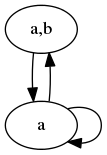
\includegraphics[width=0.2\textwidth]{Figures/kripke4.png}
  \caption{Estructura de Kripke del modelo.}
  \label{fig:kripke4}
\end{figure}

\begin{figure}[H]
  \centering
  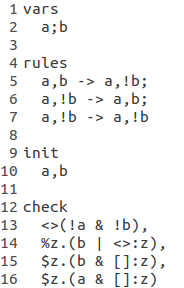
\includegraphics[width=0.35\textwidth]{Figures/modeloMC2-1.png}
  \caption{Ejemplo de descripción MC2.}
  \label{fig:MC2-1}
\end{figure}

Se puede ver que las reglas describen precisamente las tres transiciones del sistema. Aquellas proposiciones que no varian su valor de un estado al siguiente, se las puede obviar en la parte derecha de la regla como se ve en la figura \ref{fig:MC2-2}. Esta descripción es equivalente a la anterior. Intuitivamente podemos pensar la parte izquierda de la regla como el estado corriente y la parte derecha como el siguiente estado, pero en realidad podemos representar mas de una transición con una sola regla. Por ejemplo, la descripción de la figura \ref{fig:MC2-3} modela el sistema de la figura \ref{fig:kripke5}. Al omitir $a$ en la parte izquierda de las reglas, estamos diciendo que las mismas se cumplen tanto si vale como si no vale $a$.

\begin{figure}[H]
  \centering
  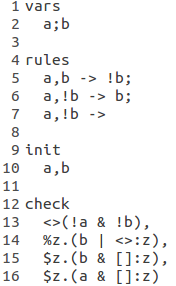
\includegraphics[width=0.33\textwidth]{Figures/modeloMC2-2.png}
  \caption{Ejemplo de descripción MC2 usando azucar sintáctico.}
  \label{fig:MC2-2}
\end{figure}

\begin{figure}[H]
  \centering
  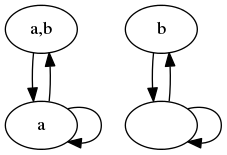
\includegraphics[width=0.4\textwidth]{Figures/kripke5.png}
  \caption{Estructura de Kripke del nuevo modelo.}
  \label{fig:kripke5}
\end{figure}

\begin{figure}[H]
  \centering
  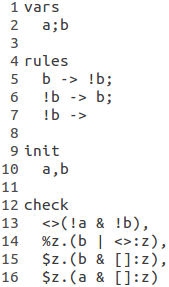
\includegraphics[width=0.33\textwidth]{Figures/modeloMC2-3.png}
  \caption{Ejemplo de descripción MC2 con más de una transición por regla.}
  \label{fig:MC2-3}
\end{figure}

En la sección $check$ se puede ver que hay cuatro propiedades descritas en cálculo-$\mu$, que son las siguientes: $\Diamond (\neg a \land \neg b)$, $\mu z. (b \lor \Diamond z)$, $\nu z. (b \land \Box z)$, y $\nu z. (a \land \Box z)$. Al ejecutar el verificador con la descripción de la figura \ref{fig:MC2-1}, el resultado va a ser el conjunto de propiedades que el modelo haya satisfecho, en este caso $\mu z. (b \lor \Diamond : z)$ y $\nu z. (a \land \Box : z)$, ya que existe un camino en donde $b$ vale en algun momento, y $a$ vale siempre en todo camino. Evidentemente $'\$'$ representa a $\nu$ y $'\%'$ representa a $\nu$. Cabe destacar también que al anteponer $':'$ a una cadena estamos haciendo referencia a una variable y no a una proposición.

\subsection{Semántica formal}

En esta sección vamos a formalizar las nociones descriptas en la sección anterior. Vamos a necesitar usar operaciones de OBDDs, para lo cual tenemos NOT, AND, OR, NULL(True si no hay modelos para este OBDD \cite{Waldmann:6} ), EXISTS, OBDD-TRUE y OBDD-FALSE. La semántica de una descripción MC2 es la siguiente:\\
\\
$[[\ vars\ D\ rules\ C\ init\ E\ check\ P ]]_{m}\ =\ [F\ |\ F \in P\ \land\ NULL\ (NOT\ inst\ E\ ([[F]]_{f}\ [[C]]_{c}\ assoc-init))]$ \\

Es decir, de todas las fórmulas en $P$ solo nos quedamos con aquellas que al instanciarlas con los valores de $init$ siempre da como resultado $True$. La semántica de una declaración está dada por la siguiente función: \\
\\
\begin{align*}
[[p]]_{d}\ &=\ (p,False) \\
[[D0;D1]]_{d}\ &=\ [[D0]]\ ++\ [[D1]] \\
\end{align*}

Una declaración da como resultado un ambiente, es decir, una lista de proposiciones con sus valores asociados ($False$ en principio). A continuación tenemos la función que denota la semántica de los modelos, un modelo es la disyunción de una o más reglas, a su vez, una regla es una disyunción de todas las transiciones que genera, donde una transición es una conjunción de los OBDDs generados por la evaluación de los ambientes del estado corriente y el siguiente (en el siguiente estado todas las proposiciones deben estar primadas).

\begin{align*}
[[C;D]]_{c}\ &=\ [[C]]_{c}\ OR\ [[D]]_{c} \\
[[E0->E1]]_{c}\ &=\ [[E0]]_{e}\ AND\ [[E1]]_{e'} \\
\end{align*}

La evaluación de un ambiente esta dada por las funciones $[[E]]_{e}$ y $[[E]]_{e'}$, donde la única diferencia entre estas funciones es que la segunda prima a las proposiciones. La semántica de un ambiente da como resultado la conjunción de las proposiciones del mismo con paridad acorde a sus valores asociados.

\begin{align*}
[[(p,True)]]_{e}\ &=\ OBDD_{p} \\
[[(p,False)]]_{e}\ &=\ NOT\ OBDD_{p} \\
[[E0++E1]]_{e}\ &=\ [[E0]]_{e}\ AND\ [[E1]]_{e} \\
\end{align*}

\begin{align*}
[[(p,True)]]_{e'}\ &=\ OBDD_{p'} \\
[[(p,False)]]_{e'}\ &=\ NOT\ OBDD_{p'} \\
[[E0++E1]]_{e'}\ &=\ [[E0]]_{e'}\ AND\ [[E1]]_{e'} \\
\end{align*}

Por ultimo, la semántica de las fórmulas, es la vista en el capítulo 3. M es el modelo del sistema (un OBDD). Assoc es una función que asocia cada variable relacional con un OBDD. La operación EXISTS de los OBDD toma un conjunto de variables y las elimina existencialmente de un OBDD.

\begin{align*}
[[p]]_{f}\ M\ assoc\ &=\ OBDD_{p} \\
[[:X]]_{f}\ M\ assoc\ &=\ assoc\ X \\
[[!F]]_{f}\ M\ assoc\ &=\ NOT\ ([[F]]_{f}\ M\ assoc)\\
[[F \& G]]_{f}\ M\ assoc\ &=\ ([[F]]_{f}\ M\ assoc)\ AND\ ([[G]]_{f}\ M\ assoc)\\
[[F | G]]_{f}\ M\ assoc\ &=\ ([[F]]_{f}\ M\ assoc)\ OR\ ([[G]]_{f}\ M\ assoc)\\
[[<>F]]_{f}\ M\ assoc\ &=\ EXISTS\ x'\ :\ M\ AND\ ([[F]]_{f}(x')\ M\ assoc) \\
[[[]F]]_{f}\ M\ assoc\ &=\ [[!<>!F]]_{f}\ M\ assoc \\
[[\%X.F]]_{f}\ M\ assoc\ &=\ FIX\ F\ assoc\ OBDD-FALSE \\
[[\$X.F]]_{f}\ M\ assoc\ &=\ FIX\ F\ assoc\ OBDD-TRUE \\
\end{align*}

\section{Diseño e implementación}

En esta sección vamos a aclarar detalles del diseño y la implementación del verificador de modelos MC2. La herramienta esta implementada en el lenguaje funcional Haskell, y se interpreta con ghc. La misma está compuesta por los módulos $Types$, $Mu$, $MuEval$, $Model$, $ModelEval$, $Main$, y usa dos modulos externos, $OBDD$ \cite{Waldmann:6} (provee la estructura con sus operaciones) y $ParseLib$ \cite{Hutton:10} (tiene utilidades de parsing).

\subsection{Tipos en MC2}

En $MC2$ tenemos proposiciones atómicas ($AP$) representadas por cadenas, cada una tiene asociada un valor lógico ($True$ o $False$), para lo cual existe un tipo $Env$ (ambiente) que consta de una lista de pares de proposiciones atómicas y sus valores lógicos asociados. Un valor de tipo $Env$ representa el estado del sistema en un momento dado. Tambien definimos el tipo $VName$ como sinónimo de cadenas, pero este tipo lo usamos para hacer referencia a variables relacionales. También hemos definido en este modulo el tipo $Assoc$ como una función Assoc: $VName -> OBDD AP$. $OBDD AP$ hace referencia al tipo de OBDDs donde las variables de sus nodos estan representadas con cadenas (AP). Assoc es un tipo que se utiliza en la semántica de las fórmulas de cálculo-$\mu$, este representa una función que toma el nombre de una variable y devuelve el valor asociado (representado por un OBDD).

\subsection{Descripción del modelo en MC2}

Hay dos modulos dedicados a la descripción del modelo. Uno es $Model$, el cuál contiene la definición de la sintaxis de las declaraciones y comandos, y  sus correspondientes $parsers$. El otro módulo es $ModelEval$, este contiene las funciones $ceval$, $deval$ y $eeval$ correspondientes a los evaluadores de comandos, declaraciones y ambientes respectivamente, además de algunas funciones auxiliares. La función $deval$ toma una declaración y un ambiente con proposiciones a inicializar (se usa en la sección $init$ unicamente), y a partir de estos genera el ambiente inicial del sistema. La función $eeval$ transforma un ambiente en una OBDD-conjunción como se vió en la semántica de ambientes.

\subsection{Cálculo-$\mu$ en MC2}

Similarmente tenemos dos modulos dedicados al Cálculo-$\mu$. Uno es $Mu$, el cuál contiene la definición de la sintaxis, y adicionalmente también contiene el $parser$, y un $printer$. El otro módulo es $MuEval$, este contiene la función $check$ que, dada una fórmula, un modelo (OBDD) y la función $Assoc$, evalua la fórmula y devuelve el OBDD correspondiente a su semántica. Al ser funcional la implementación, toda la información necesaria para computar un resultado debe ser pasada como parámetro, por lo que la función $check$ también toma dos parámetros extra, necesarios para reescribir los nombres de las proposiciones atómicas del OBDD por sus respectivas versiones primas (cuando es necesario verificar algo sobre el siguiente estado). Además $MuEval$ contiene algunas funciones auxiliares como $fix$, la cual se utiliza en el cálculo de puntos fijos.

\subsection{Módulo principal}

El módulo $Main$ contiene el $parser$ de descripciones MC2, su evaluador y varias funciones auxiliares para la lectura de archivos.